
% Variablen laden
% Basisdaten (Titelseite, etc.)
\newcommand{\mytitle}{Titel der Arbeit}
\newcommand{\mypaper}{Diplomarbeit}
\newcommand{\myduedate}{01. Juli 2011}
\newcommand{\mytutor}{Prof. Foo Bar}
\newcommand{\myauthor}{John Doe}
\newcommand{\myid}{012345678}
\newcommand{\myemail}{john.doe@example.com}
\newcommand{\mylocation}{Localhost}
\newcommand{\mydegree}{Master of Arts}
\newcommand{\myschool}{University XYZ}
\newcommand{\myclass}{JG}

% Meta-Keywords der Arbeit fürs PDF
\newcommand{\mykeywords}{}

%% Statische strings
% Zitate
\newcommand{\strcompare}{vgl.}
\newcommand{\strsee}{}
\newcommand{\strsource}{Quelle}
\newcommand{\strcitefiguremodified}{Modifiziert nach}
\newcommand{\strcitefiguredata}{Eigene Darstellung, Daten entnommen aus}
\newcommand{\strcitefigureown}{Eigene Darstellung}

% Titelseiten
\newcommand{\strclass}{Jahrgang}
\newcommand{\strobtaindegree}{zur Erlangung des akademischen Grades}
\newcommand{\strsubmittedwhere}{Eingereicht an der}
\newcommand{\strauthor}{Verfasser}
\newcommand{\strtutor}{Betreuer}
\newcommand{\strduedate}{Abgabedatum}

% Überschriften
\newcommand{\strglossary}{Abkürzungsverzeichnis}
\newcommand{\strbibliography}{Quellenverzeichnis}

% Erste Konfigurationen einbinden
\documentclass[
    a4paper,
    twoside=false,
    fontsize=11pt,
%   DIVcalc,            % Bei Problemen mit den Seitenrändern testweise aktivieren
%   BCOR=5mm,           % Zusätzlicher Binderand links
    parskip=half,       % Absatzabstand statt Einrückung neuer Zeile
    headsepline,        % Linie nach der Kopfzeile
%   bigheadings,        % "grössere" Überschriften
    numbers=noenddot,
    bibliography=totoc,
    listof=totoc,
    tocflat,
    pagesize=pdftex
]{scrreprt}

\usepackage{cmap}                       % Für ein durchsuchbares PDF
\usepackage[T1]{fontenc}
\usepackage{ucs}                        % UTF8 initialisieren
\usepackage[utf8x]{inputenc}            % UTF8 benutzen

\usepackage{csquotes}
\usepackage[english,ngerman]{babel}     % Einstellungen Deutsch, aber zuvor Englisch geladen, um einige Einstellungen auf default zu setzen

\usepackage{lmodern}
\usepackage{palatino}                   % Schriftsatz
    \renewcommand{\sfdefault}{lmss}         % default Sans Serif Font; lmss == lmodern Sans Serif

\usepackage{ifpdf}
\usepackage{url}                        % URLs formatieren
\usepackage{graphicx}                   % Grafikpackage
\usepackage[usenames]{color}            % Farben
\usepackage{lipsum}                     % mit \lipsum Blindtext einfügen
\usepackage{texlogos}                   % TeX Logos
\usepackage{eurosym}                    % EUR Symbol
\usepackage{setspace}                   % Zeilenabstand
\usepackage{microtype}                  % Optischer Randausgleich
\usepackage{romannum}                   % Römische Zahlen mit \romannum oder \Romannum
\usepackage{pdfsync}                    % PDF Sync

\usepackage{tocstyle}
    \usetocstyle{allwithdot}

\usepackage{geometry}                   % Setzt die Seitenabstände auf Vorgabe vom Leitfaden
    % zusätzlich verwendbar: headsep=10mm, footskip=12mm
    % abstand kopfzeile-text, abstand text-fusszeile
    \geometry{a4paper, left=35mm, right=30mm, top=30mm, bottom=30mm}

    \setcounter{tocdepth}{4}            % Gliederungstiefe im Inhaltsverzeichnis; Jarz´sche Vorgabe ist "vollständig"
    \setcounter{secnumdepth}{3}         % Gliederungstiefe bis zu der Nummeriert wird

\usepackage{scrhack}
\usepackage{listings}                   % Für Listings (einbinden eines Quellcodes)
    % Festlegungen für Listings
    \definecolor{ListingBG}{rgb}{0.85,0.92,0.94}
    \lstset{
        language=PHP,                       % Programmiersprache; z.B.: PHP, C, C++, HTML, Java, SQL, etc. (see "listings"-Package for more Information)
        numbers=left,                       % Zeilennummerierung auf der linken Seite
        numberstyle=\scriptsize,            % Zeilennummerierung kleine Schriftgröße
        stringstyle=\ttfamily,              % Courier Schriftart für Strings
        showstringspaces=false,             % In Strings keine Backspace zeichen
        numbersep=5pt,                      % Abstand der Zeilennummern zum Code
        basicstyle=\small,                  % Schriftgröße small
        breakatwhitespace=true,
        breaklines=true,
        tabsize=4,                          % Tabulator wie in Visual C++
        commentstyle=\color{green},         % Kommentarfarbe
        keywordstyle=\color{blue}\bfseries, % Keywörterfabe
        backgroundcolor=\color{ListingBG},
    }

% \renewcommand{\name}[Anzahl]{Definition #1}
\makeatletter
\let\NAT@parse\undefined
\newcommand{\BibTeX}{\bibtexlogo}   % Kompatiblität
\makeatother

% Zitationen in Fußnoten erlauben
\usepackage[round,authoryear,sort]{natbib}  % für Darstellung der Literaturverweise im Text

% Herausgestellte Zitate Kursiv
\newenvironment{zitat}%
{\begin{quote}\itshape}%
{\end{quote}}%

% Itemabstände bei Listen verringert
\let\origitemize\itemize
\def\itemize{\origitemize\itemsep-4pt}
\let\origenumerate\enumerate
\def\enumerate{\origenumerate\itemsep-4pt}
\let\origdescription\description
\def\description{\origdescription\itemsep-4pt}

% Schrift in der Kopfzeile
\setkomafont{pagehead}{\scriptsize\slshape}         % Schrift in der Kopfzeile

% Literaturverzeichnis in Quellenverzeichnis umbenennen
% entsprechend der gewählten Sprache
\addto{\captionsngerman}{
    \renewcommand{\bibname}{\strbibliography}       % statt "Literaturverzeichnis"
    % \renewcommand{\figurename}{Abb.}              % Abbildung durch Abb. ersetzen
    % \renewcommand{\tablename}{Tab.}               % Tabelle durch Tab. ersetzen
}%

% Formatierungen für Bild- und Tabellenunterschriften
\usepackage[format=plain,                           % Bildunterschriften
    justification=centerlast,                       % Die letzte Zeile wird zentriert
    labelfont={small,bf,it},                        % Abbildung <Nr> wird small, fett und italic gesetzt
    textfont={small,singlespacing,it},              % Der Text wird small und italic mit einfachem Zeilenabstand gesetzt
    width={0.8\textwidth}
]{caption}

% Tabellen: http://www.unix-ag.uni-kl.de/~fischer/blog/20070411_Tabellen_in_LaTeX/
\usepackage{multirow}
\usepackage{multicol}
\usepackage{ifthen}

\newcommand{\forloop}[5][1]{%
\setcounter{#2}{#3}%
\ifthenelse{#4}{#5\addtocounter{#2}{#1}%
\forloop[#1]{#2}{\value{#2}}{#4}{#5}}%
{}}

\newcounter{crcounter}

\newcommand{\compensaterule}[1]{%
\forloop{crcounter}{1}{\value{crcounter} < #1}%
{\vspace*{-\aboverulesep}\vspace*{-\belowrulesep}}}

\newcommand{\multirowbt}[3]{\multirow{#1}{#2}%
{\compensaterule{#1}#3}}

% durchgehende Nummerierung bei Fussnoten, Abbildungen und Tabellen
\usepackage{chngcntr}
    \counterwithout{footnote}{chapter}
    \counterwithout{table}{chapter}
    \counterwithout{figure}{chapter}


% Commands laden (z.B. Zitate)
%% Zitate

% \footcitev[S.23f]{Autor2011} -> Fußnote: vgl. Autor, 2011, S.23f
\newcommand{\footcitev}[2][]{\footnote{~\citealp[\strcompare][#1]{#2}}}

% \footcites[S.23f]{Autor2011} -> Fußnote: siehe Autor, 2011, S.23f
\newcommand{\footcites}[2][]{\footnote{~\citealp[\strsee][#1]{#2}}}

% \citev[S.23f]{Autor2011} -> (vgl. Autor, 2011, S.23f)
\newcommand{\citev}[2][]{~(\citealp[\strcompare][#1]{#2})}

% \cites[S.23f]{Autor2011} -> (siehe Autor, 2011, S.23f)
\newcommand{\cites}[2][]{~(\citealp[\strsee][#1]{#2})}

% \citefigure[S.23f]{Autor2011} -> (Quelle: Autor, 2011, S.23f)
\newcommand{\citefigure}[2][]{~(\citealp[\strsource:][#1]{#2})}

% \citefiguremodified[S.23f]{Autor2011} -> (Modifiziert nach Autor, 2011, S.23f)
\newcommand{\citefiguremodified}[2][]{~(\citealp[\strcitefiguremodified][#1]{#2})}

% \citefiguredata[S.23f]{Autor2011} -> (Eigene Darstellung, Daten entnommen aus Autor, 2011, S.23f)
\newcommand{\citefiguredata}[2][]{~(\citealp[\strcitefiguredata][#1]{#2})}

% \citefigureown -> Eigene Darstellung
\newcommand{\citefigureown}{~(\strcitefigureown)}


%============================================================
% Weitere Konfigurationen und Abkürzungen
%============================================================
%% 	PDF und Links formatieren
\usepackage[pdftex,pagebackref,pdfa]{hyperref}
\pdfcompresslevel=1 %% ZLib Komprimierung: 0==none; 1==fastest; 9==best
\pdfimageresolution=1200 %% Bilder in 600dpi ; Standard ist 300dpi
\pdfminorversion=5

\hypersetup{plainpages=false,
	pdftitle={\mytitle},
	pdfauthor={\myauthor},
	pdfsubject={\mypaper},
	pdfcreator={},
	pdfproducer={},
	pdfkeywords={\mykeywords},
	colorlinks=true,
	linkcolor=black,
	citecolor=black,
	urlcolor=black,
	a4paper,
	breaklinks=true,
%	linktocpage=true, % verlinkt nur die Seitenzahlen im tableofcontents, da bei Umbruch der Link kaputt gehen kann
	bookmarksopen=true,
	bookmarksnumbered=true,
	bookmarksopenlevel=1,
	pdfmenubar=true,
	pdfwindowui=true,
	pdfview=FitV,
	pdfstartview=Fit,
	pdffitwindow=true
}

% Rückreferenzentext zur Literatur im Quellenverzeichnis (nach hyperref!)
\renewcommand*{\backreftwosep}{ und~}
\renewcommand*{\backreflastsep}{ und~}
\renewcommand*{\backref}[1]{}
\renewcommand*{\backrefalt}[4]{%
\ifcase #1 %
 (nicht zitiert).%
\or
 (zitiert auf Seite~#2).%
\else
 (zitiert auf den Seiten~#2).%
\fi
}

% Glossar / Abkürzungsverzeichnis / Symbolverzeichnis; nach hyperref
\usepackage[
nonumberlist, %keine Seitenzahlen anzeigen
toc,          %Eintrag im Inhaltsverzeichnis
]{glossaries}

% Länge der gepunkteten Linie
\setlength{\glslistdottedwidth}{.2\linewidth}

% Den Punkt am Ende jeder Beschreibung deaktivieren
\renewcommand*{\glspostdescription}{}

% Weitere Formatierungen
\glsSetSuffixF{\nohyperpage{f.}}
\glsSetSuffixFF{\nohyperpage{ff.}}

% Kompilieranweisungen
\makeindex          % Sortieren
\makeglossaries     % Abkürzungsverzeichnis erstellen

% Abkürzungen
% \newacronym{cpu}{CPU}{Central Processing Unit}
% im Text dann:  ... erreichen wir bei \gls{VerweismarkeText}-Systemen ...
\newacronym{ad}{AD}{Active Directory}
\newacronym{ldap}{LDAP}{Lightweight Directory Access Protocol}
    % Glossar, Abkürzungsverzeichnis und/oder Symbolverzeichnis

%============================================================
% Dokumentanfang und Titelei
%============================================================
\begin{document}
    %============================================================
% Äussere Titelseite (Schmutztitel)
%============================================================
\begin{titlepage}
	\thispagestyle{empty}
%	\setcounter{page}{-2}

\begin{center}
	\hspace{1cm}
\vfill

\begin{minipage}{0.99\textwidth}
\begin{center}
\onehalfspacing
\Huge \textsf{\textbf{\mytitle}}
\end{center}
\end{minipage}

\vfill
	\hspace{1cm} \\ \vspace{2em}
\vfill
	\hspace{1cm} \\ \vspace{2em}
\vfill

\textbf{\textsf{\LARGE{%
\myauthor \\
\mypaper \\
}}}%

\vspace{1em}
\textsf{\LARGE{%
\strclass~\myclass \\
}}%

\end{center}

%============================================================
% Leerseite plus Innere Titelseite
%============================================================
	\newpage
	\thispagestyle{empty}
	\hspace{1cm}
	\newpage
	\thispagestyle{empty}
\begin{center}

\mbox{
\includegraphics[width=4.5cm]{img/logo_title.png}}

\vfill

%{\Huge \textsf{\textbf{\mytitle}}}
\begin{minipage}{0.99\textwidth}
\begin{center}
\onehalfspacing
\Huge \textsf{\textbf{\mytitle}}
\end{center}
\end{minipage}

\vfill

{\LARGE \textsf{\textbf{\\ \mypaper}}}

\large
\strobtaindegree \\
\mydegree

\vspace{1em}

\strsubmittedwhere \\
\myschool\\
\myclass

\vspace{1em}

\strauthor \\
\myauthor \\
\myid \\
\myemail \\

\vspace{1em}

\strtutor \\
\mytutor

\vspace{1.5em}

\strduedate \\
\myduedate

\end{center}
\end{titlepage}

\pagenumbering{roman}
    \setcounter{page}{2}

\chapter*{Eidesstattliche Erklärung}

\textsl{Ich erkläre hiermit, dass ich die vorliegende Diplomarbeit selbständig und ohne fremde Hilfsmittel verfasst und in der Bearbeitung und Abfassung keine anderen als die angegebenen Quellen oder Hilfsmittel benutzt sowie wörtliche und sinngemäße Zitate als solche gekennzeichnet habe. Die vorliegende Diplomarbeit wurde noch nicht anderweitig für Prüfungszwecke vorgelegt.}
\vspace{1cm}

\makebox[0.45\textwidth]{%
\mylocation, den \today
}%

\vspace{2cm}

\rule{0.45\textwidth}{0.3pt} \\
\makebox[0.45\textwidth]{%
{\myauthor}
}%


%============================================================
% Vorspann mit kleinen römischen Seitenzahlen
%============================================================
    \tableofcontents
        \clearpage
    \listoftables
    \listoffigures
	\lstlistoflistings
    \printglossary[toctitle=Abkürzungsverzeichnis,style=listdotted,title=Abkürzungsverzeichnis]     % Glossar, Abkürzungsverzeichnis und/oder Symbolverzeichnis ausgeben
\clearpage
\onehalfspacing
    \chapter*{Kurzfassung}

Lorem ipsum dolor sit amet, consectetuer adipiscing elit. Ut purus elit, vestibulum ut, placerat ac, adipiscing vitae, felis. Curabitur dictum gravida mauris. Nam arcu libero, nonummy eget, consectetuer id, vulputate a, magna. Donec vehicula augue eu neque. Pellentesque habitant morbi tristique senectus et netus et malesuada fames ac turpis egestas. Mauris ut leo. Cras viverra metus rhoncus sem. Nulla et lectus vestibulum urna fringilla ultrices. Phasellus eu tellus sit amet tortor gravida placerat. Integer sapien est, iaculis in, pretium quis, viverra ac, nunc. Praesent eget sem vel leo ultrices bibendum. Aenean faucibus. Morbi dolor nulla, malesuada eu, pulvinar at, mollis ac, nulla. Curabitur auctor semper nulla. Donec varius orci eget risus. Duis nibh mi, congue eu, accumsan eleifend, sagittis quis, diam. Duis eget orci sit amet orci dignissim rutrum.

\chapter*{Executive Summary}

Lorem ipsum dolor sit amet, consectetuer adipiscing elit. Ut purus elit, vestibulum ut, placerat ac, adipiscing vitae, felis. Curabitur dictum gravida mauris. Nam arcu libero, nonummy eget, consectetuer id, vulputate a, magna. Donec vehicula augue eu neque. Pellentesque habitant morbi tristique senectus et netus et malesuada fames ac turpis egestas. Mauris ut leo. Cras viverra metus rhoncus sem. Nulla et lectus vestibulum urna fringilla ultrices. Phasellus eu tellus sit amet tortor gravida placerat. Integer sapien est, iaculis in, pretium quis, viverra ac, nunc. Praesent eget sem vel leo ultrices bibendum. Aenean faucibus. Morbi dolor nulla, malesuada eu, pulvinar at, mollis ac, nulla. Curabitur auctor semper nulla. Donec varius orci eget risus. Duis nibh mi, congue eu, accumsan eleifend, sagittis quis, diam. Duis eget orci sit amet orci dignissim rutrum.


%============================================================
% Hauptteil
%============================================================
\clearpage
\pagestyle{headings}
\onehalfspacing
\pagenumbering{arabic}
    \chapter{Beispielcontent}

\section{Quellenverweise}

Die Sache mit dem Zitieren ist eine Geschichte voller Missverständnisse. Zuerst gibt es da nämlich die Unterscheidung zwischen Kurz- und Langzitaten.

Ein sogenanntes Kurzzitat ist ein Verweis im Text, der auf Autorenname(n) und Jahreszahl besteht \citev[S.72]{BIBTEXKEYBook}. Es ist uns freigestellt, ob wir wie hier den Literaturverweis direkt in den Text einbauen wie in einschlägiger Literatur meist anzutreffen\cites[S.72]{BIBTEXKEYBook}, oder -- wie es dem Herrn Jarz ganz gut gefällt -- über Fußnoten\footcites[S.39]{BIBTEXKEYarticle} unsere Quellenangaben machen. Für die Sache mit den Fußnoten habe ich deshalb auch etwas eingebaut\footcitev[S.39]{BIBTEXKEYarticle}.

Ein Lang- oder Vollzitat hingegen ist eine komplette Quellenangabe, so wie wir es ins Quellenverzeichnis hinten im Dokument schreiben. So etwas stünde immer in einer Fußnote, ist meines Erachtens aber überflüssig, da wir ja ein Quellenverzeichnis haben. Daher sollten Verweise im Text ausreichen.

Um die Formatierung des Quellenverzeichnis übrigens müssen wir uns nicht weiter kümmern, solange alle relevanten Daten über JabRef in der Literaturdatenbank eingetragen sind, \BibTeX~ sei Dank.


\section*{Sectionüberschrift ohne Nummerierung}
Hier eine Sectionüberschrift ohne Nummerierung: Das geht auch mit anderen Überschriften, und liegt an dem angefügten Stern im Code.


\section{Liste mit Punkten}
\begin{itemize}
\item Punkt1 mit Text
\item Noch etwas
\item Und was ganz anderes
\item Ebenso ein Schmarrn
\end{itemize}


\section{Nummerierte Liste}
\begin{enumerate}
\item Punkt1 mit Text
\item Noch etwas
\item Und was ganz anderes
\item Ebenso ein Schmarrn
\end{enumerate}


\section{Liste Description}
\begin{description}
\item[davor] Punkt1 mit Text
\item[lalala] Noch etwas
\item[huhuu] Und was ganz anderes
\item[undso] Ebenso ein Schmarrn
\end{description}


\section{Ein Bildchen}
Ein Verweis auf ein Bild (wie z.B. Abbildung~\ref{fig:texlogo} auf Seite~\pageref{fig:texlogo}) im geschriebenen Text wird immer per Nummerierung gemacht, nie mit einem Doppelpunkt nach einem Satz der vor dem Bild zu stehen hat.

\begin{figure}[ht]
        \centering
            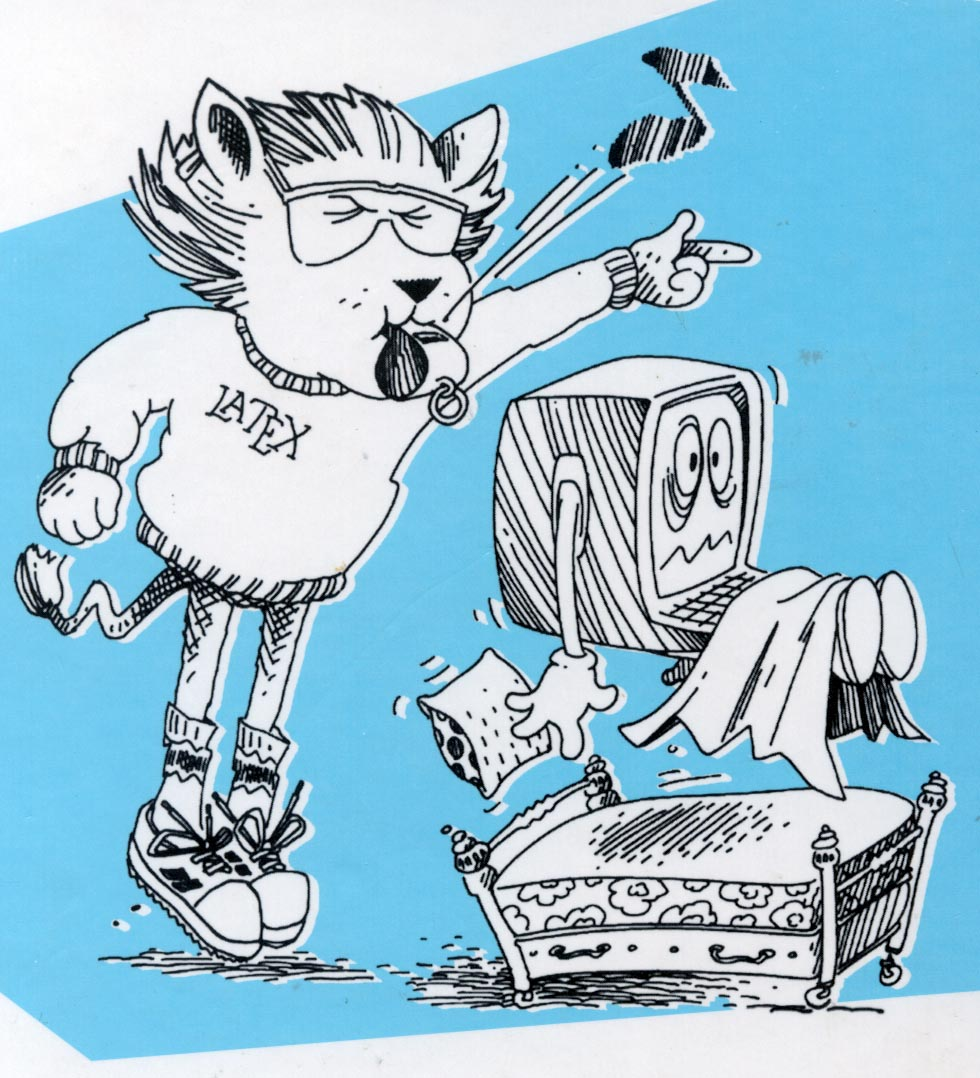
\includegraphics[width=0.35\textwidth]{img/latex.jpg}    % Bild relativ zur Textbreite skalieren
            \caption[\LaTeX~Logo]
                {Und dieser Text hier erscheint schlussendlich direkt unterhalb des Bildes. Daher kann hier durchaus auch etwas mehr stehen\citefigureown.}
            \label{fig:texlogo}
\end{figure}

\begin{figure}[ht]
        \centering
            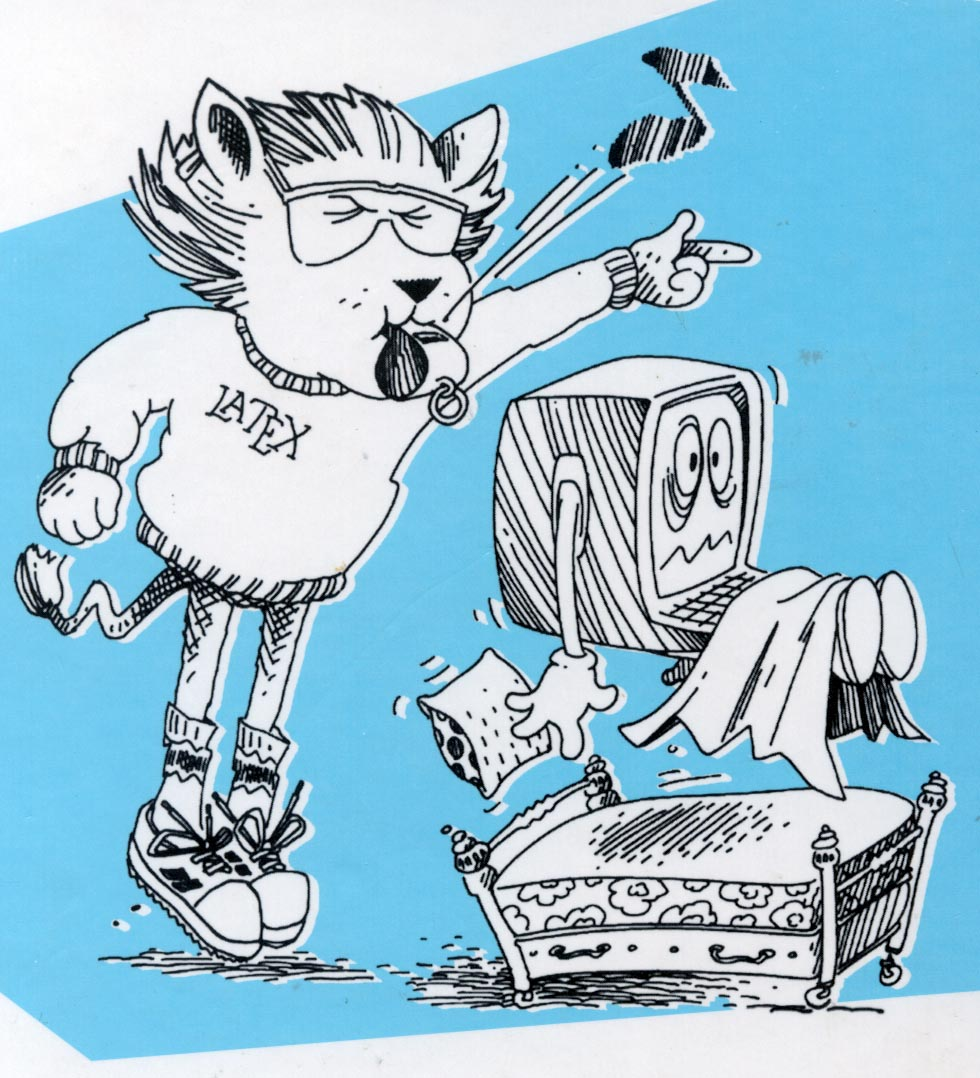
\includegraphics[width=0.35\textwidth]{img/latex.jpg}    % Bild relativ zur Textbreite skalieren
            \caption[\LaTeX~Logo]
                {Ein Bild aus externer Quelle\citefigure[S.39]{BIBTEXKEYarticle}.}
            \label{fig:texlogo2}
\end{figure}

\begin{figure}[ht]
        \centering
            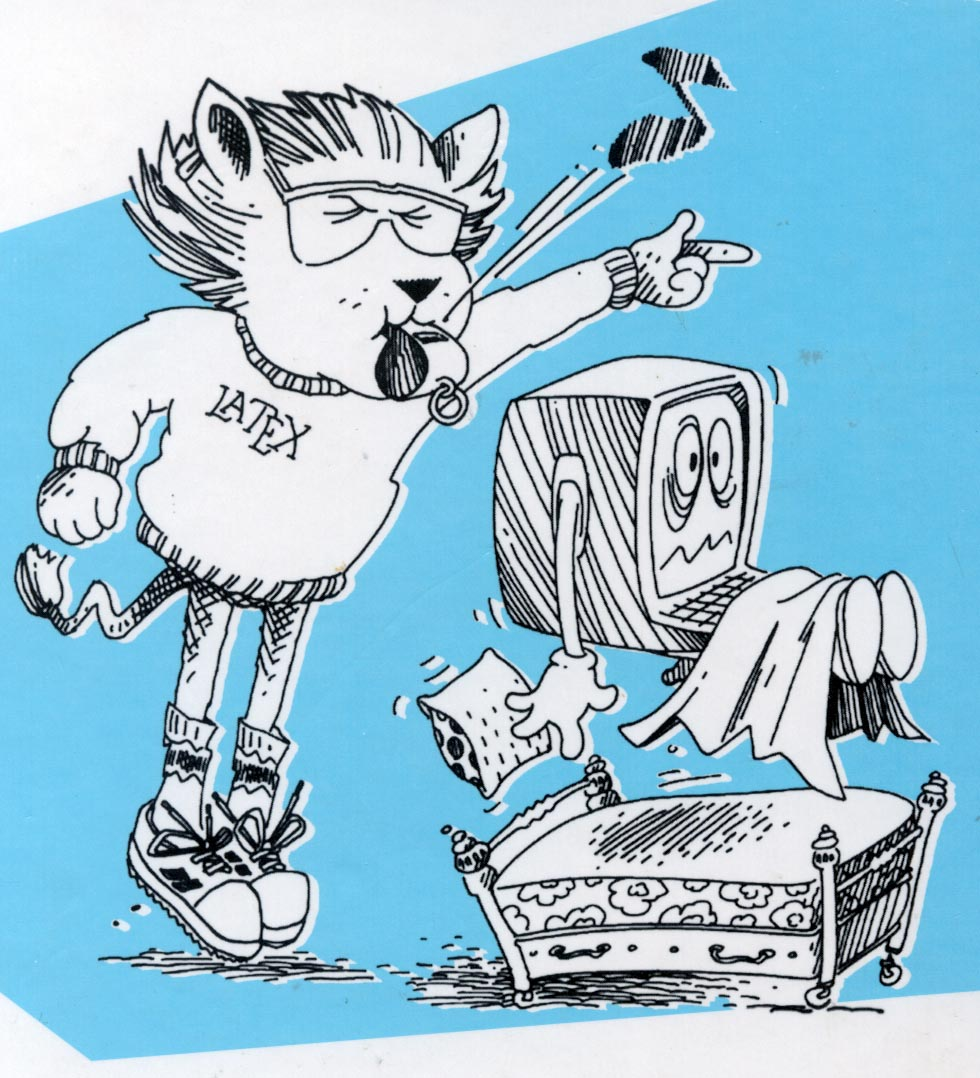
\includegraphics[width=0.35\textwidth]{img/latex.jpg}    % Bild relativ zur Textbreite skalieren
            \caption[\LaTeX~Logo]
                {Modifiziertes Bild aus externer Quelle\citefiguremodified[S.39]{BIBTEXKEYarticle}.}
            \label{fig:texlogo3}
\end{figure}

\begin{figure}[ht]
        \centering
            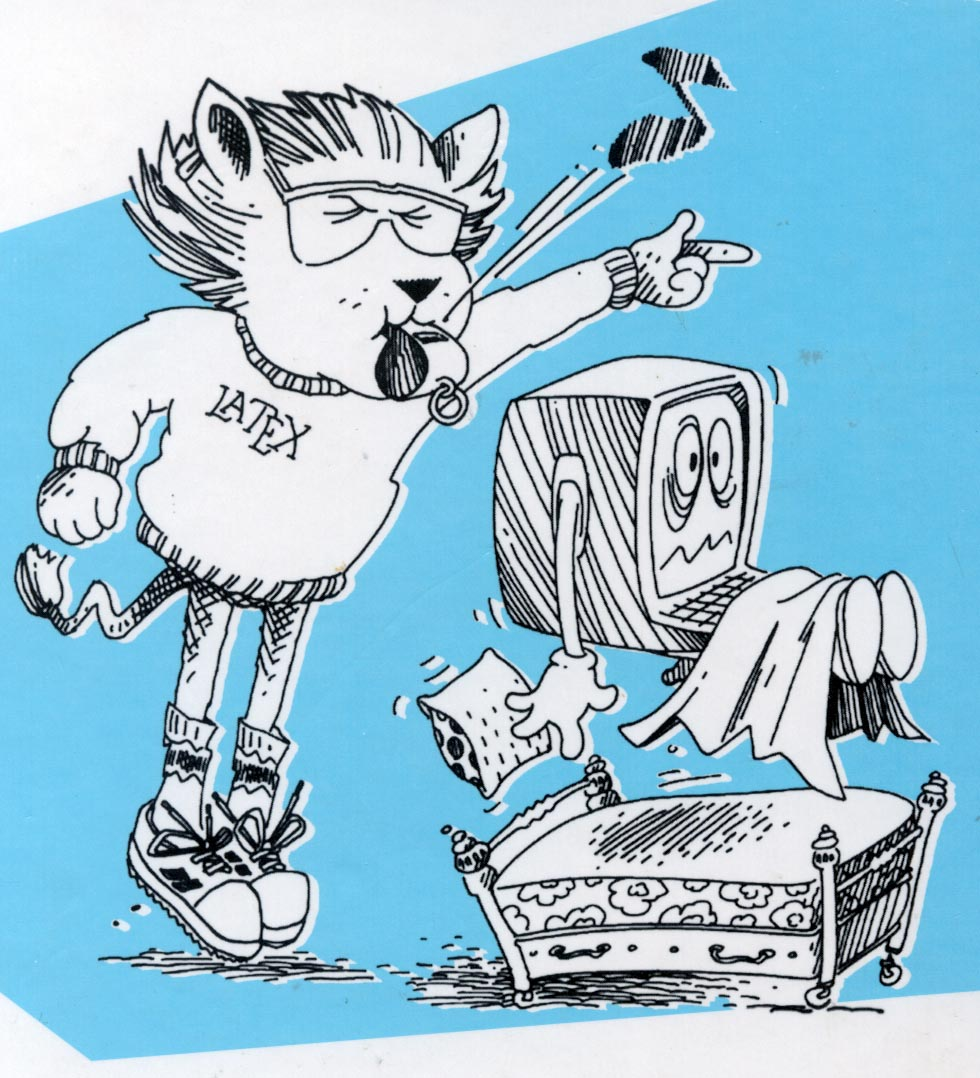
\includegraphics[width=0.35\textwidth]{img/latex.jpg}    % Bild relativ zur Textbreite skalieren
            \caption[\LaTeX~Logo]
                {Eigene Darstellung mit externen Daten\citefiguredata[S.39]{BIBTEXKEYarticle}.}
            \label{fig:texlogo4}
\end{figure}


\section{Textformatierungen}

In diesem Text werden ein paar wenige, aber übliche Formatierungen dargestellt,
je nachdem ob man \textbf{fett} drucken möchte, \textit{kursiv} oder \underline{unterstrichen}, aber auch die \emph{Hervorhebung}
gewisser Terme könnte von Vorteil sein.

Obacht! Fettdruck im normalen Fließtext sollte NIEMALS nötig sein\footcitev[S.112]{BIBTEXKEYarticle}.

Gerade für Sourcecode bietet sich die \texttt{Schreibweise mit fester Laufweite} an. Für Namen würde sich eventuell auch
die Verwendung echter \textsc{Kapitälchen} anbieten, für welche ganz explizit \LaTeX~sehr bekannt ist.

Termini technici werden oft auch \textsl{slanted} oder \textit{kursiv} dargestellt, mit kleinen Unterschieden.


\section{Ein herausgestelltes Zitat}
\begin{zitat}
    "`Graecum te, Albuci, quam Romanum atque Sabinum,
    municipem Ponti, Tritani, centurionum,
    praeclarorum hominum ac primorum signiferumque,
    maluisti dici. Graece ergo praetor Athenis,
    id quod maluisti, te, cum ad me accedis, saluto:
    'chaere,' inquam, 'Tite!' lictores, turma omnis chorusque:
    'chaere, Tite!' hinc hostis mi Albucius, hinc inimicus."'
\end{zitat}


\section{Eine einfache Tabelle}

Tabellen werden in der table-Umgebung gesetzt, um auch als Tabellen erkannt zu werden (siehe Tabelle~\ref{tab:WerkCicero} auf Seite~\pageref{tab:WerkCicero}). Fügte man hier beispielsweise das Bild oder PDF einer Excel-Tabelle ein, würde es ebenso  als Tabelle geführt.

\begin{table}[!t]
	\centering
	\begin{tabular}{cll}\hline\hline
	Jahr & Originaltitel & engl. Titel \\ \hline
	84 BC & De Inventione & About the composition of arguments \\
	55 BC & De Oratore & About oratory \\
	54 BC & De Partitionibus Oratoriae & About the subdivisions of oratory \\
	52 BC & De Optimo Genere Oratorum & About the Best Kind of Orators \\
	46 BC & Paradoxa Stoicorum & Stoic Paradoxes \\
	46 BC & Brutus & For Brutus \\
	46 BC & Orator ad M. Brutum & About the Orator, dedicated to Brutus \\
	45 BC & De Fato & On Fate \\
	44 BC & Topica & Topics of argumentation \\ \hline\hline
	\end{tabular}
	\caption[Dies ist der Kurztitel fürs Verzeichnis]{Und hier steht dann derjenige Text, welcher direkt unterhalb der Tabelle zu finden ist.}
	\label{tab:WerkCicero} 	% Textmarke
\end{table}


\section{Verweise und Referenzen}
\label{sec:references}

Indem man \verb+\label+ im Code vergibt, kann man mit \verb+\ref+ direkt darauf verweisen, und mit \verb+\pageref+ sogar die Seitennummer angeben. Als Rückgabewert kommt bei Bildern und Tabellen die jeweilige Nummerierung, bei Überschriften die Gliederungsnummer. An dieser Stelle verweise ich auf Überschrift~ \ref{sec:references}, welche auf Seite~ \pageref{sec:references} steht.

Die Tilde im Code bedeutet, dass an dieser Stelle ein fester Leerraum steht, der nicht getrennt werden darf.


\section{Sourcecode einfügen}
Sourcecode wird in der \verb+\listings+ Umgebung gesetzt, mit vielen Möglichkeiten der Formatierung. Es wird fast jede Programmiersprache explizit unterstützt. Näheres unter \url{http://www.pvv.ntnu.no/~berland/latex/docs/listings.pdf}

\begin{lstlisting}[caption=Dies ist ein PHP Beispiel]{Beispiel}
public function delete()
{
    if ($_SESSION['login'] == 'test') {
        $this->db_delete('bbericht', 'IDbbericht', $_GET['id'], '');
    } else {
        $this->sec_msg();
    }
}
\end{lstlisting}    %$ (Dieses Dollarzeichen ist nur eingefügt, da der Editor sonst denkt man hätte hier noch eine mathematische Formel-Umgebung offen, die zwischen Dollarzeichen gesetzt würde)


\section{Silbentrennung}

Sollte \LaTeX~wirklich einmal Probleme mit der Silbentrennung eines unbekannten Wortes haben, kann man über hyphenation
die Trennweise bekannt machen, oder auch das Trennen von Wörtern verbieten.
\begin{verbatim}
\hyphenation{er-go-no-mic}
\hyphenation{fortran}
\end{verbatim}
 "`fortran"' darf nie getrennt werden, "`ergonomic"' an den angegebenen Stellen


\section{Mathematische Formeln}

\LaTeX~ ist berühmt für seine einzigartigen Fähigkeiten im Umgang mit mathematischen Formeln.

Dabei gibt es die einfache Variante kurze Formeln wie $1+1=3$ direkt in den Text einzufügen, oder auch komplexere Formeln herausgehoben darzustellen, die dann auch nummeriert werden:

\begin{equation}%Beginn der Formel
t-t_{0}=\sqrt{\frac{l}{g}}\int_{0}^{\varphi}{\frac{d\psi}{\sqrt{1-k^{2}\sin^{2} {\psi}}}} = \sqrt{\frac{l}{g}} F(k,\varphi)
\end{equation}%Ende der Formel

\begin{equation}%Beginn der Formel
u(x,t)= 8 \frac{k_{1}^{2}e^{\alpha_{1}} + k_{2}^{2}e^{\alpha_{2}} + (k_{1}-k_{2})^{2}e^{(\alpha_{1}+ \alpha_{2})} \left[2 + \frac{1}{(k_{1} + k_{2})^{2}} ( k_{1}^{2}e^{\alpha_{1}} + k_{2}^{2}e^{\alpha_{2}}) \right]}{\left[1+e^{\alpha_{1}} + e^{\alpha_{2}} + \left(\frac{k_{1} - k_{2}}{k_{1}+k_{2}} \right)^{2} e^{\alpha_{1}+ \alpha_{2}} \right]^{2}}
\end{equation}%Ende der Formel


\section{Anführungszeichen}
Ein Satz mit "`Anführungszeichen"'.
Ein Satz mit französischen \frqq Anführungszeichen\flqq.
Ein Satz mit \textit{halben} französischen \frq Anführungszeichen\flq.


\section{Umlaute}
Sollten mal Probleme mit Umlauten auftreten, kann man sich mit den nativen Umlautzuweisungen behelfen:
\"a, \"A, \"o, \"O, \"u, \"U


\section{Abkürzungen}
Werden im Text Abkürzungen wie \gls{ad} für Active Directory benutzt, müssen diese vorher in der glossary-Datei definiert werden.
Von den zuvor definierten Abkürzungen werden aber nur diejenigen wirklich im Verzeichnis aufgeführt, welche auch im Texr verwendet wurden.
\gls{ad} wurde bereits verwendet mit \verb+\gls{ad}+. Ebenso \gls{ldap}, aber CD wurde hier nicht als Code eingefügt, und fehlt daher im Verzeichnis.

Das besondere dabei: Bei der ersten Verwendung im Text wird die Abkürzung automatisch ausgeschrieben! Auch wird das Verzeichnis automatisch alphabetisch sortiert.


\section{Gliederungsebenen}
Die oberste Ebene ist das chapter, hier befinden wir uns gerade in einer section.
\subsection{Subsection}
\subsubsection{Subsubsection}
Spätestens hier sollte man mit Nummerierung aufhören!
\paragraph{Paragraph}
Und wer hier noch Nummerierung will, ist krank ;-)
\subparagraph{Subparagraph}

\section{Blindtext mit \LaTeX}
\lipsum


%============================================================
% Abspann mit Anhängen und Quellenverzeichnis
%============================================================
\appendix                       % Ab hier Nummerierung A, B, ...
\clearpage
\onehalfspacing
    \input{content/appendix.tex}

\newpage
\singlespacing
    %\nocite{*}                 % NUR FÜR TESTZWECKE!!! Damit provoziert man ein vollständiges Literaturverzeichnis ALLER bib-Einträge; normalerweise werden nur die im Text wirklich benutzten Quellen ins Verzeichnis aufgenommen
    \bibliographystyle{natdin}  % Literaturverzeichnis nach DIN
    \bibliography{bibliography} % Datei der Jabref Bibliotheksdatei .bib

%============================================================
\end{document}
